\section{Introduction}



Movement variability is an inherent feature within a person and between persons
\cite{newell1993variability}. Recently, Herzfeld et al. \cite{Herzfeld2014}
conducted experiments to argue that movement variability is not only noise but a
source of movement exploration which at certaing point is becoming a source
of movement explotation.
With this in mind, we have found that there is little research in the area of
human-robot interaction that is focused on the quantification of movemennt variablity.


%
% Blake et al. \cite{Blake2007} reviewed studies of perception of human motion
% in which is stated that
%   % that one contribution to the percpetion of human motion is
% % motor experience
% the ability of people to perceive the actions of other people
% is based on acumulated experiences of planning and executing self-produced
% activites.
% %% REF: MOTORIC CONTRIBUTIONS TO PERCEPTION OF HUMAN MOTION \cite{Blake2007}
%



% Understading the perceptual, motoric, affective and neural mechanisms
% of perception of human motion has been
% which is the ability of


...I AM READING THESE PAPERS TO COMPLETE THE INTRODUCTION:
Perception of Human Motion \cite{Blake2007}.
Pigeons and humans use action and pose information to categorize complex human behaviors
\cite{Qadri201716}. The visual perception of velocity \cite{Brown1931}.
Implied Dynamics Biases the Visual Perception of Velocity \cite{LaScaleia2014}.
Attention to body-parts varies with visual preference and verb--effector associations \cite{Boyer2017}.
Comparing Biological Motion Perception in Two Distinct Human Societies \cite{Pica2011}

% Motion perception: from phi to omega \cite{Rose967}



\section{METHOD}

\subsection{Reconstructed State Space}
In this work we follow the notation employed in \cite{Uzal2011}.
The purpose of time-delay embedding, also known as Takens's Theorem,
is to reconstruct the topological properties of an unknown $M-$dimensional
state space $s(t)$ from a $1-$dimensional measurement $x(t)$ in order to
reconstruct an $N-$dimensional embedding space.
The time-delay embedding assumes that the time series is a sequence $x(t)=h(s(t))$,
where $h: S \rightarrow \mathbb{R}^M$ is a measurement function on the unknown
dynamical system, being $x(t)$ observable (Figure \ref{fig:takens_theorem}).

\begin{figure}[!htb]
\centering
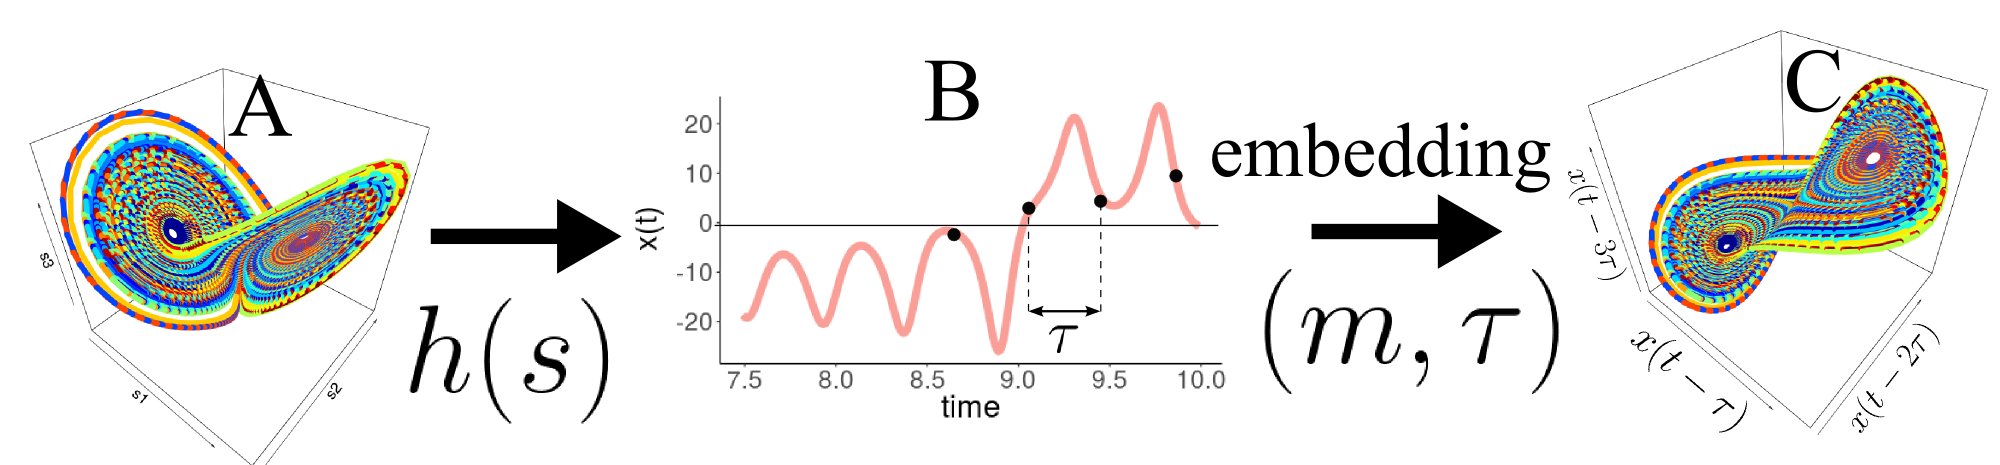
\includegraphics[width=0.45\textwidth]{figures/reconstructed_state_space/fig}
\caption[PA]{A. $M-$dimensional complex system $s(t)$; B. $1-$dimensional measurament
$x(t)$; and  C. $N-$dimensional complex system $v(t)$ where $M \geq N $}
\label{fig:takens_theorem}
\end{figure}

Thus, the time delay reconstruction in $m$ dimensions with a time delay
$\tau$ is defined as:
$\overline{x}(t) = (x(t), x(t-\tau),...,x(t-(m-1)\tau))$.
% which defines a map
% $\varPhi: S \rightarrow \mathbb{R}^m$ such that $\overline{x}(t) = \varPhi(s)$.
% $\varPsi: \mathbb{R}^m \rightarrow \mathbb{R}^n$ is
Then a further transformation can be considered
% as a more general transformation
in order to reduce
% the dimensionality of
the $m-$dimensional time-delay embedding.
For this work, we assume that the signal, $x(t)$, we are observing has been
produced by some time-varying system (that is the human body movement).
 % rather than been generated entirely at random.
The assumption that the source of the signal exhibits systematic variation
leads to the assumption that this signal should, over some time period,
exhibit a repeated pattern. What we do not know is what this time period might
be or what this repeated pattern might look like.


%
% In our work the sequence $x(t)$ is the raw data collected from an (IMU)
% for triaxial data for accelerometer ($a_{ \{ x,y,z \} }$),
% gyroscope ($g_{ \{ x,y,z \} }$) and magnetometer($m_{ \{ x,y,z \} }$) sensors.
% Then, for instance, the time-series $a_x$ with a length of
% $N$ samples is used to obtain the Time-delay embedded matrix,
% $\boldsymbol{E} a_{x}$, with $m$ rows and $N-(m-1)\tau$ columns.
% Finally, the PCA algorithm is applied so as to obtain via eigenvalues
% ($\lambda_1,\ldots,\lambda_m$), eigenvectors ($v_1,\ldots,v_m$) and
% the principal components
% ($PC_1,\ldots,PC_m$) of the time-delay embedded phase space.



\subsection{Determining the embedding parameters ($m$ and $\tau$)}
Although Takens's Theorem has been used extensively in gait
recognition and walking, running and cycling activities,
some problems are still remaining to be solved.
Sama et al. \cite{Sama2013} estimated that the minimal embedded
dimension ($m_{min}$) with False Nearest Neighbours (FNN) method.
However, Cao \cite{Cao1997} pointed out that FNN algorithm
introduces new parameters ($R_{tol}$ and $A_{tol}$) that lead
%is subject to different threshold parameters   which lead
to different results which cannot differentiate random series from
deterministic series.
Frank et al. \cite{Frank2010} proposed a grid search method to find the minimal
embedded parameters, but there are little details about their approach.
Additionally, Sama et al. \cite{Sama2013} states that the minimal embedding
parameters largely depend on the
application at hand. Thus, there is still research to be done to find the
minimal dimension parameters ($m_{min}$ and $\tau_{min}$)
to reconstruct the state space.

% \newpage
\subsection{$E1(d)$ and $E2(d)$ values}
Cao's method for computing the minimal embedding dimension is based on the
mean values of $E1(d)$ and $E2(d)$ where $d$ is the range of evaluation of the
embedding dimension. Therefore, $E1(d)$ is used to obtain the minimal
dimension $m_{min}$ to which the values of $E1(d)$ stop changing when
 $d$ comes from an attractor. $E2(d)$ values are used to distinguish
 deterministic signals from random signals in which case the $E2(d)$
 values will be approximately equal to 1 for any $d$.
Cao's method is a modified version of the FNN method, and $E1(d)$ and $E2(d)$
values are only dependant on $m$ and $\tau$ \cite{Cao1997}.
% Figures~\ref{fig:e1e2} illustrate our application of this approach,
% which is described in more detail in the Estimation of the Minimal
% Embedded Parameters section.



\section{Experiment Design}

\subsection{Head Pose Estimation}

Estimating head pose in human-robot interactions is an active area of research
% where remain
because of challenges like real-time tracking, the use of less invasive equipment
or the preparation of calibration techniques. However, Lemaignan et al. proposed a head pose estimator
using a monococular RGB webcam which is able to track a head with rotations up
to $\pm$40$^{\circ}$ horizontally and $\pm$30$^{\circ}$ vertically \cite{Lemaignan2016}.
Much recently, OpenFace, a fully open source real-time facial behavior analysis,
provides state-of-the-art performance in facial landmark motion,
head pose (orientation and motion), facial expressions, and eye gaze.
Additionally, OpenFace can operate with a simple webcam in real-time
\cite{Baltrusaitis2016}.

% Perceiving Gaze Cues with a NAO Robot \cite{Mwangi2016}


\section{Experiment}


\subsection{Hyphothesis}
In our previous experiments of a face-to-face human-humanoid imitation
activity \cite{XXX2017} where we proposed metrics to quantify the level of
imitation, we also observed (by eye) that efects like boredoom, fatigue or
level of engagment might also be a factor that influence
the way each person moves and therefore movement variability.
With this in mind, we hyphothesised that not only inertial sensors attached
to the body can provide information about movement variability
but also the head pose estimation which, we believe, will lead us to get better
understanding movement variability and therefore create
realiable metrics to measure such variability.


\subsection{Participants and Procedure}
For our pilot experiment, we only collected data for one male right-handed healthy
participant  (age 35, height 177cm, weight 85kg).
% and one female (age 25, height 150cm, weight 43).
Besides the inertial sensors attached to both the participant and the robot,
we use the head pose estimation via webcam in order to test our previous hyphothesis.
% that can lead us to understand how to estimate leves of engagement, boredoom or fatigue.
For this, we designed a pilot experiment where the user(s) imitate NAO robot' arm
movements at three speeds:
(a) 15 frames per seconds;
(b) 30 frames per seconds;
(c) and 45 frames per seconds.
Such experiment were performed for six times by the same participant
in order to test the factor of fatigue or boredoom (Figure~\ref{fig:exp}A ).

% (a) moving both arms at different speeds for short and prolonged times
% (b) moving arms alternate
% (c) either (a) or (b) with music

% With this in mind, w
We use OpenFace \cite{Baltrusaitis2016} to measure the head pose which
 let us hyphothesis that the participant is engagaed
when he/she stared the robots within certain range of movements.

% Regarding the factor of fatigue, we vary the time lenght of the performed activity
% for each of the sceneraios.
% and the similarity of movements


% Experiment set up (Figure~\ref{fig:exp}A )



\begin{figure}[!htb]
\centering
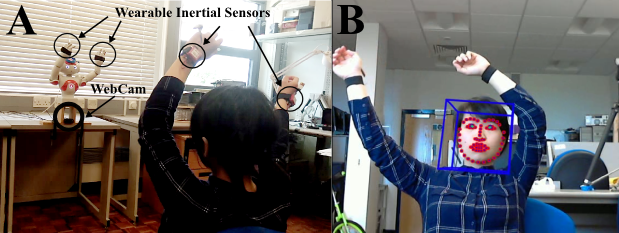
\includegraphics[width=0.45\textwidth]{figures/experiment/fig_w619h233}
\caption[PA]{A. Experimental setup: face-to-face imitation with NAO humanoid robot;
B. Head pose estimation with OpenFace \cite{Baltrusaitis2016}
}
\label{fig:exp}
\end{figure}


\section{Results}
I AM WORKING IN THIS SECTION WHERE I WILL PRESENT THE RESULTS OF
ONE PARTICIPANT PERFORMING THE ARM MOVEMENTS FOR SIX TRIALS
AT SPEEDS OF 15, 30 and 45 USING THE DATA FROM THE IMUS AND THE HEAD POSE
ESTIMATOR (Figures~\ref{fig:hpe} and \ref{fig:imus}).


\begin{figure}[!htb]
\centering
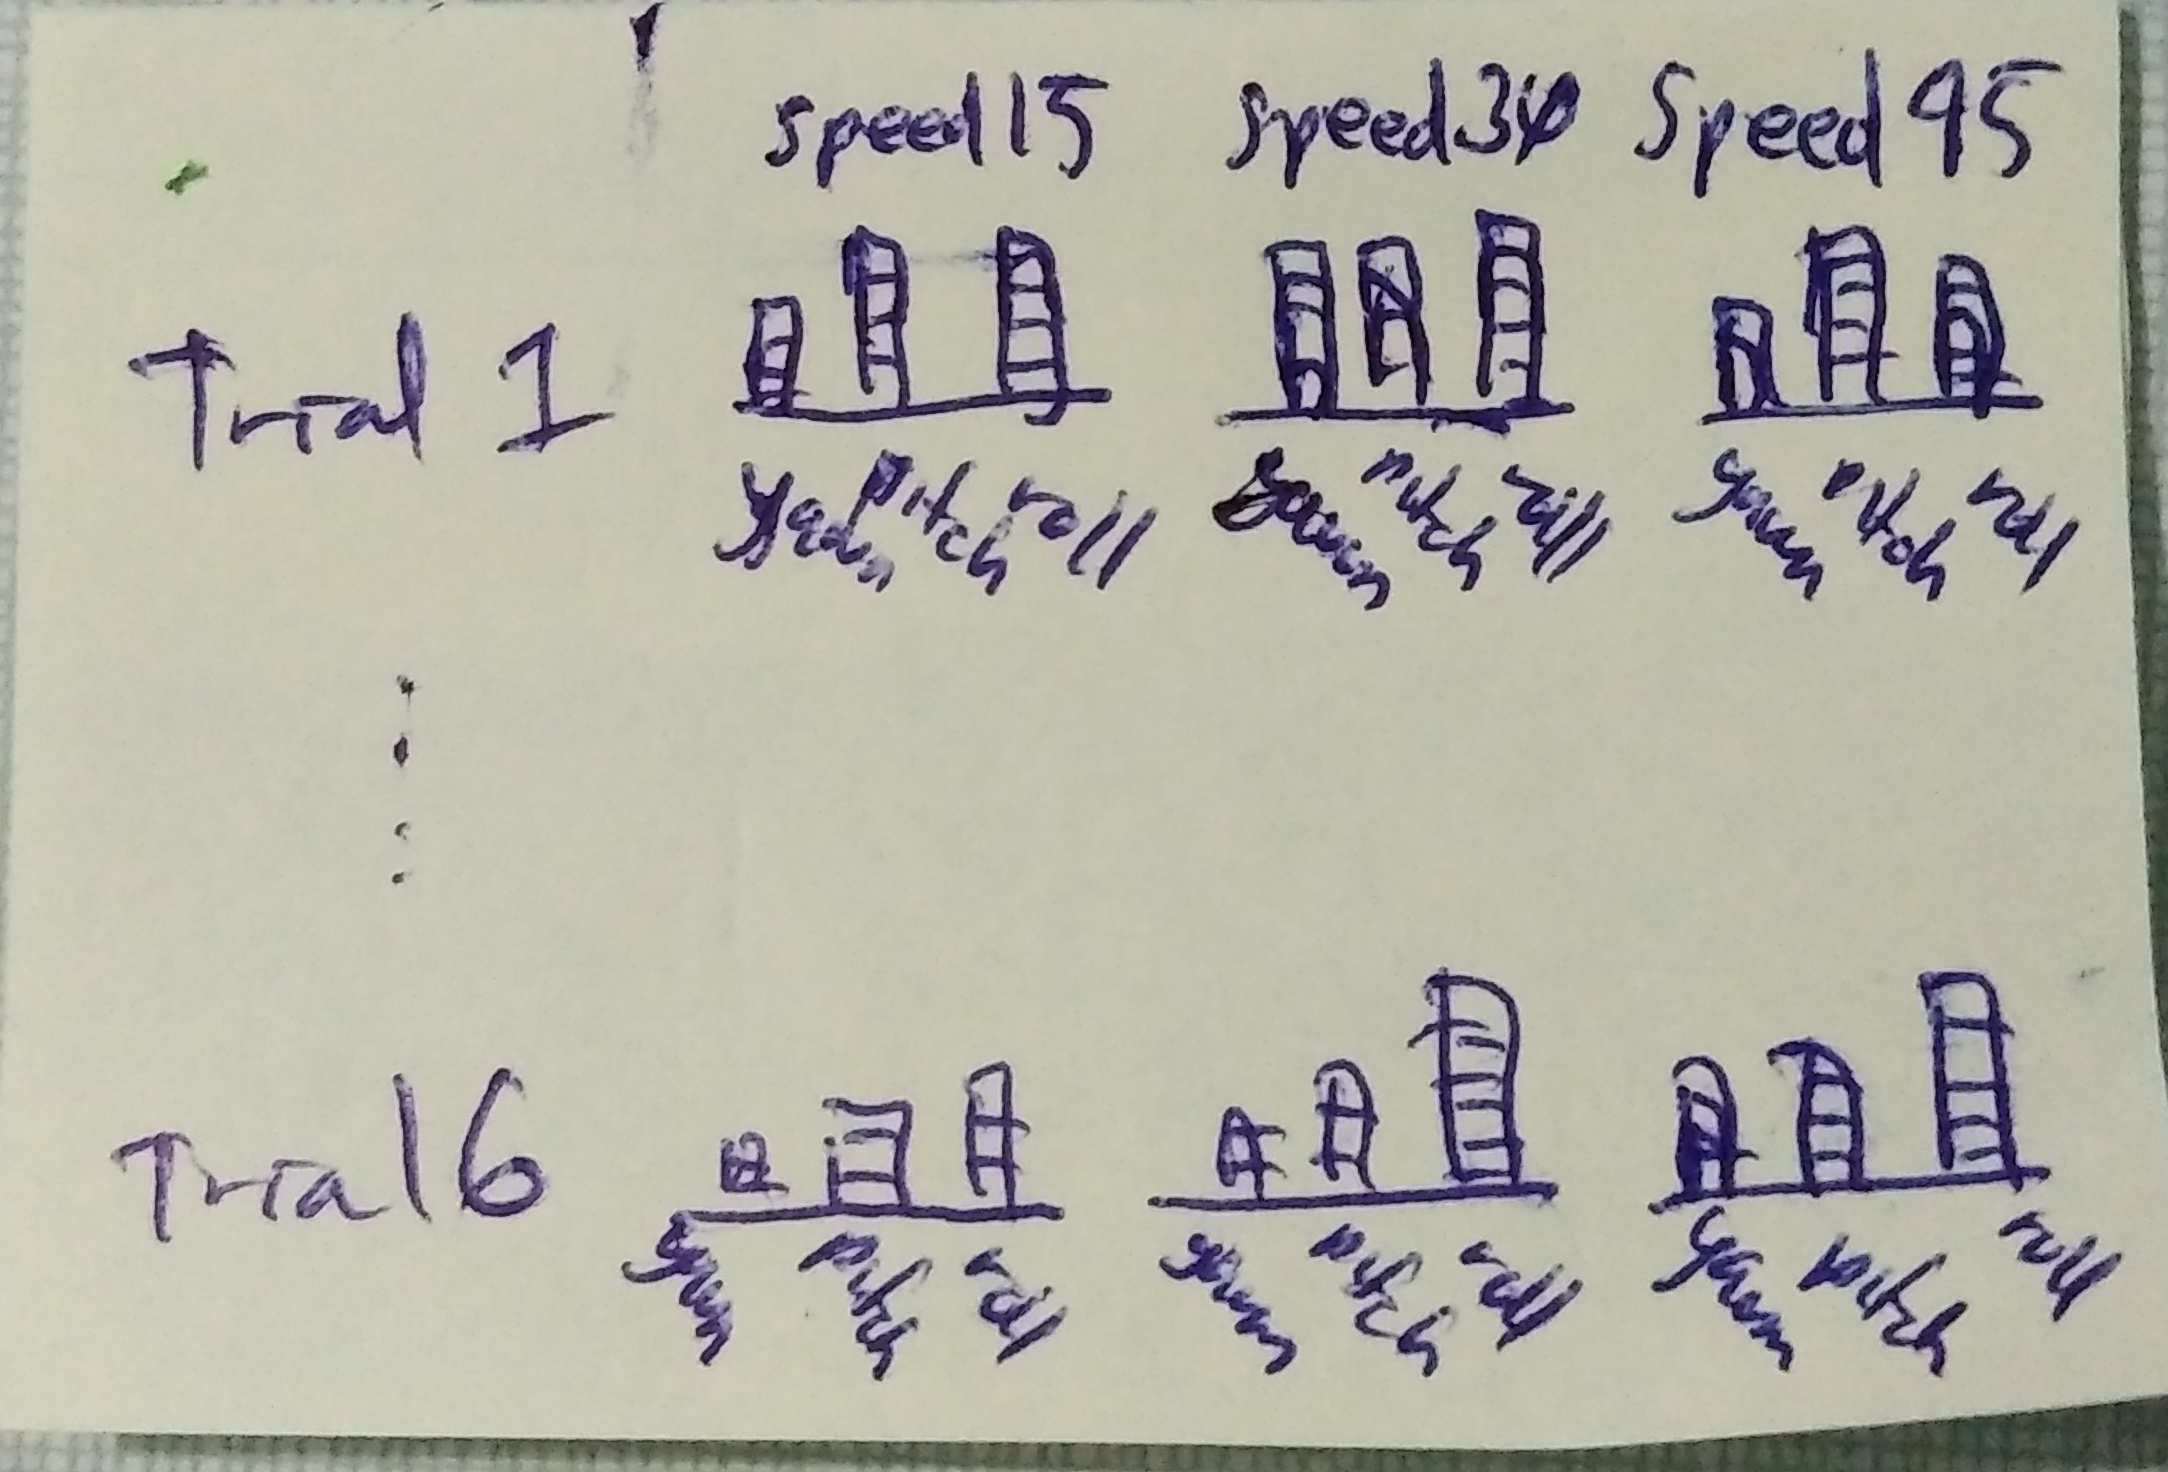
\includegraphics[width=0.45\textwidth]{figures/results/hpe}
\caption[PA]{Head Pose Estimation of six trials at three speeds 15, 30 and 45}
\label{fig:hpe}
\end{figure}



\begin{figure}[!htb]
\centering
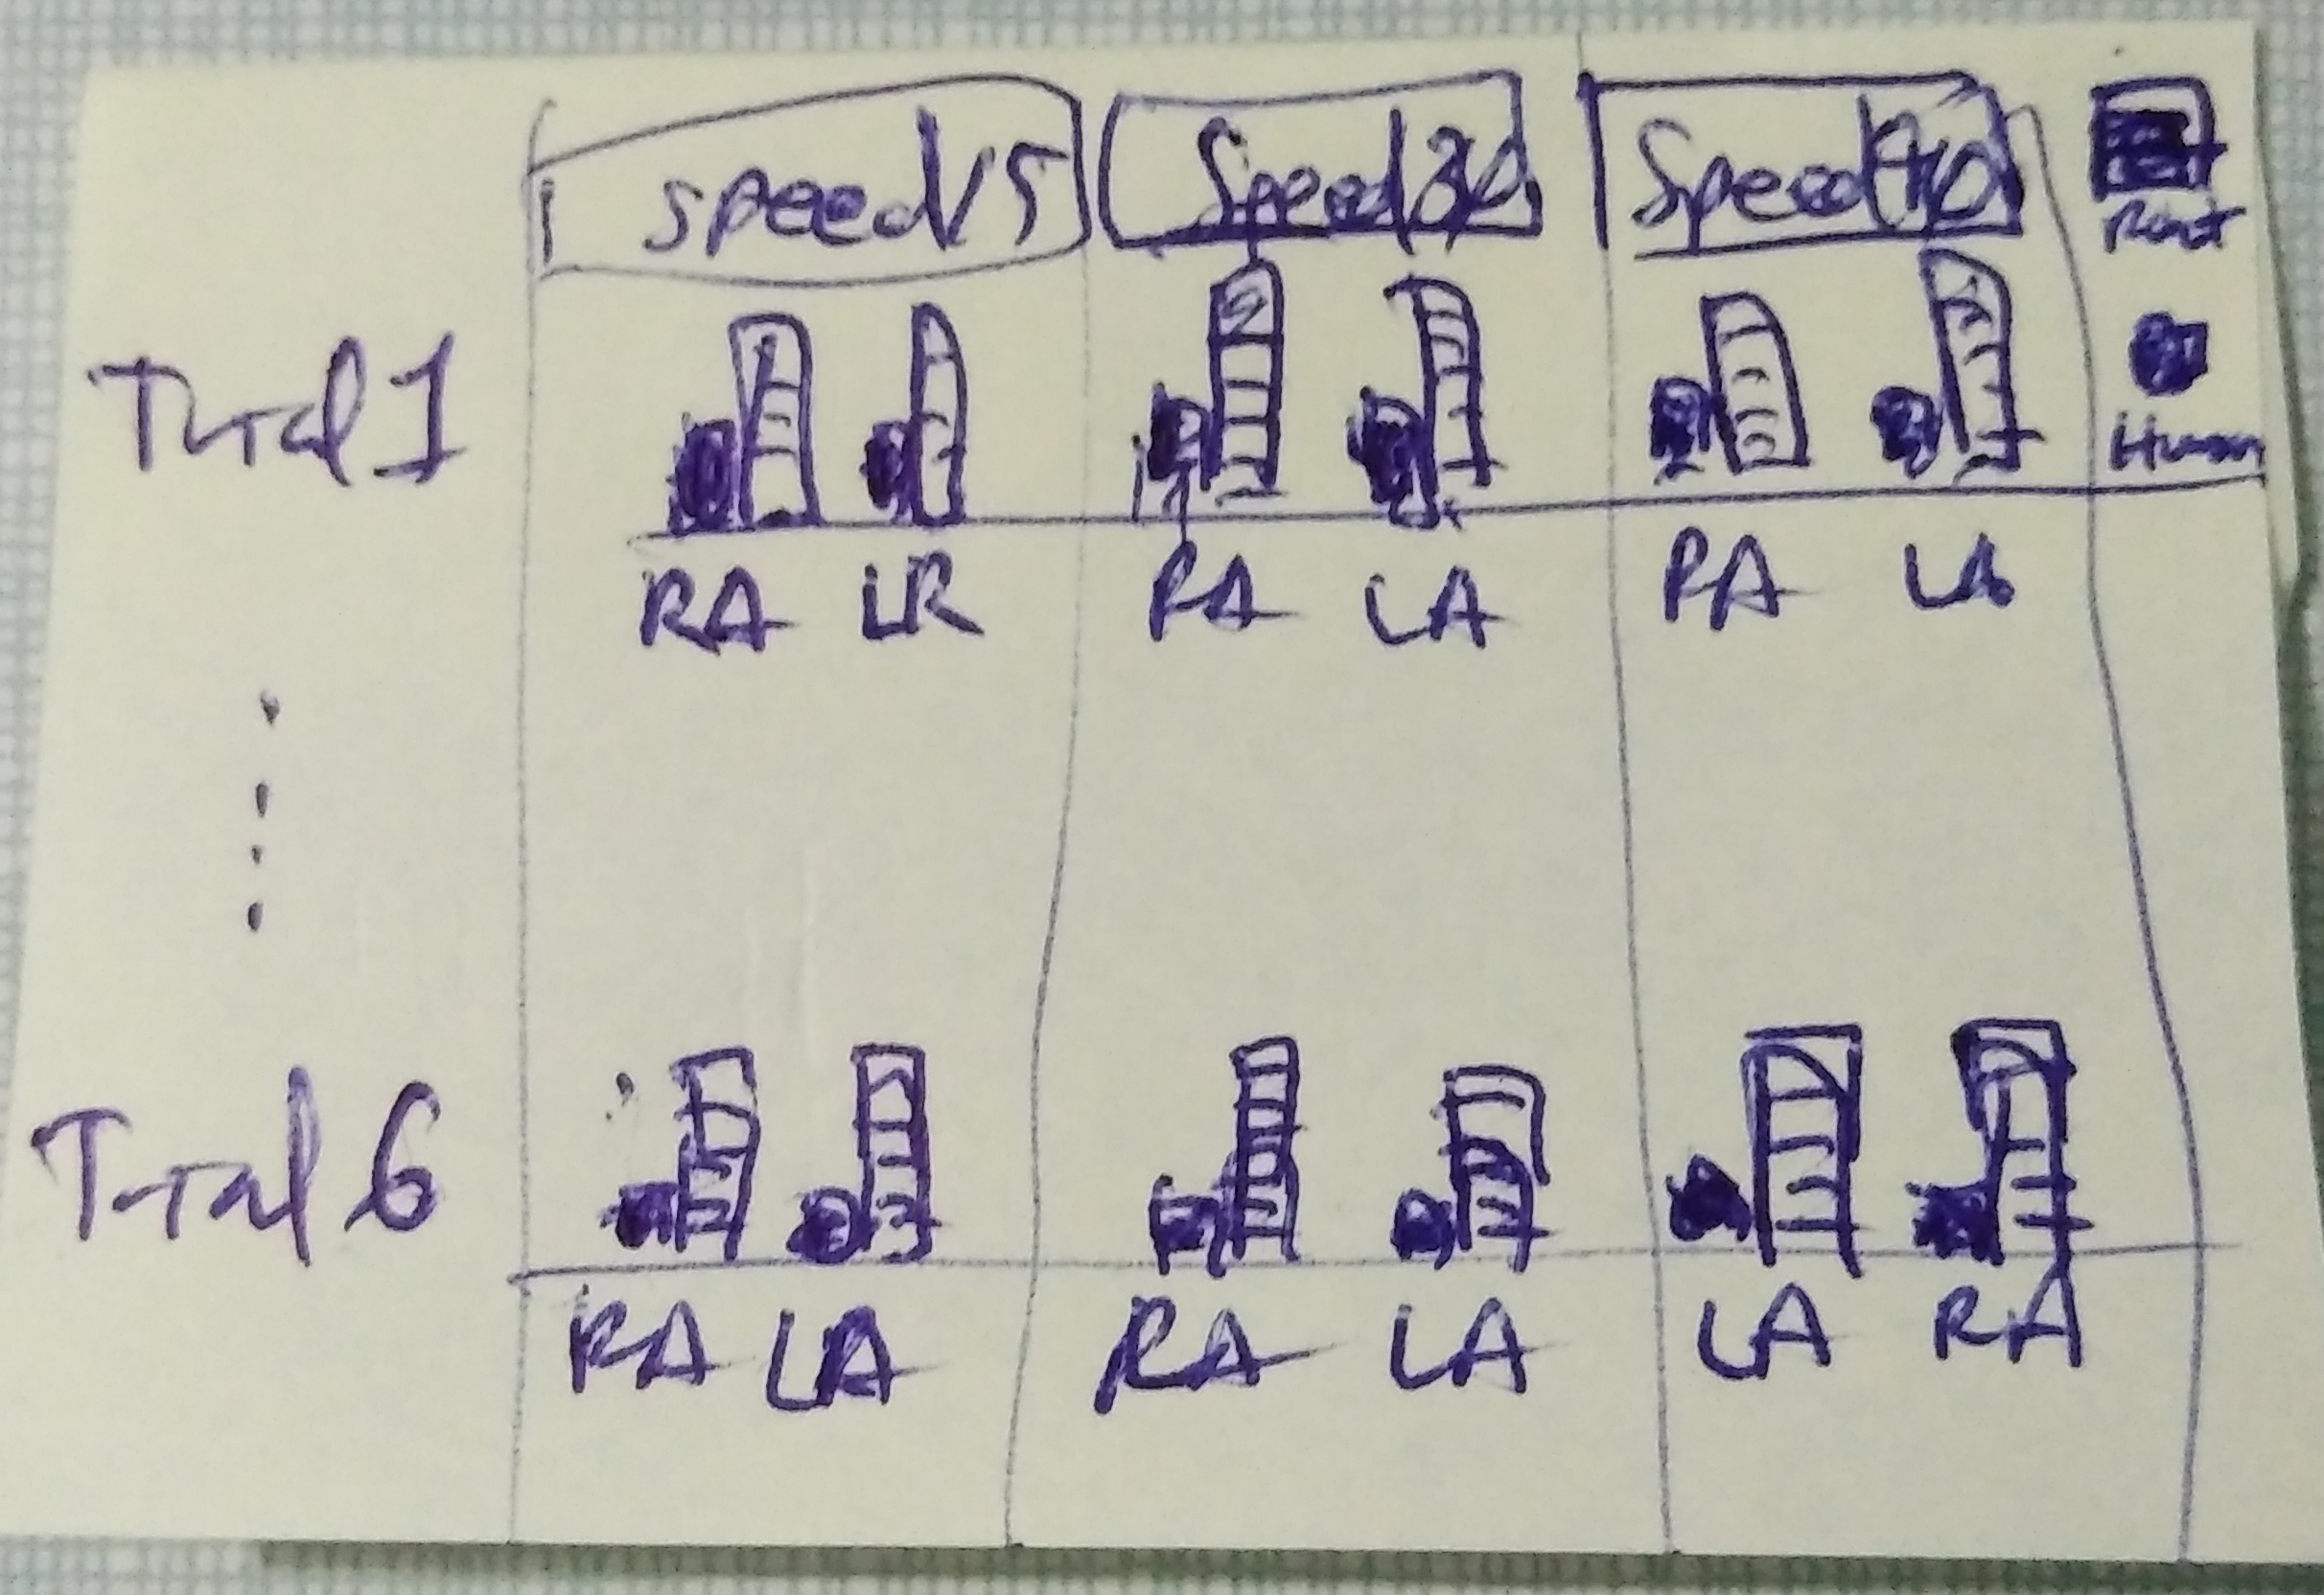
\includegraphics[width=0.45\textwidth]{figures/results/imus}
\caption[PA]{Right Arm (RA) and Left Arm (LA) from Human and robot arm movememtns
of six trials at three speeds 15, 30 and 45}
\label{fig:imus}
\end{figure}






\section{Conclusion}



In future experiments, there are three areas that we intend to investigate:
(a) provide further understanding of human movement variablity
(b) two-humans to one-humanoid and
(c) three-humans to one-humanoid interactions.

% (b) data collection from a wider range of individuals (differing gender, age and state of health)
% and from additional inertial sensors attached to the body;
% (ii) exploration of complex movements which can be performed by both persons and NAO;








\section{Conclusions}
This paragraph will end the body of this sample document.
Remember that you might still have Acknowledgments or
Appendices; brief samples of these
follow.  There is still the Bibliography to deal with; and
we will make a disclaimer about that here: with the exception
of the reference to the \LaTeX\ book, the citations in
this paper are to articles which have nothing to
do with the present subject and are used as
examples only.
%\end{document}  % This is where a 'short' article might terminate





\begin{acks}

  The authors would like to thank Dr. Yuhua Li for providing the
  matlab code of  the \textit{BEPS} method.

  The authors would also like to thank the anonymous referees for
  their valuable comments and helpful suggestions. The work is
  supported by the \grantsponsor{GS501100001809}{National Natural
    Science Foundation of
    China}{http://dx.doi.org/10.13039/501100001809} under Grant
  No.:~\grantnum{GS501100001809}{61273304}
  and~\grantnum[http://www.nnsf.cn/youngscientsts]{GS501100001809}{Young
    Scientsts' Support Program}.

    XXX gratefully acknowledges XXX for pursuing his doctoral studies at
    University of XXX. Special thanks is also extended to XXX from XXX at
    University of XXX for XXX
    acute critics and suitable comments that are helping the work to give a better
    shape to the scientific value of knowledge of my research endevours.


\end{acks}
